\beginsong{Die Internationale}[wuw={Eugène Pottier, Pierre Degeyter, 1871}, index={Wacht auf, Verdammte dieser Erde}]

\beginverse
\endverse
\centering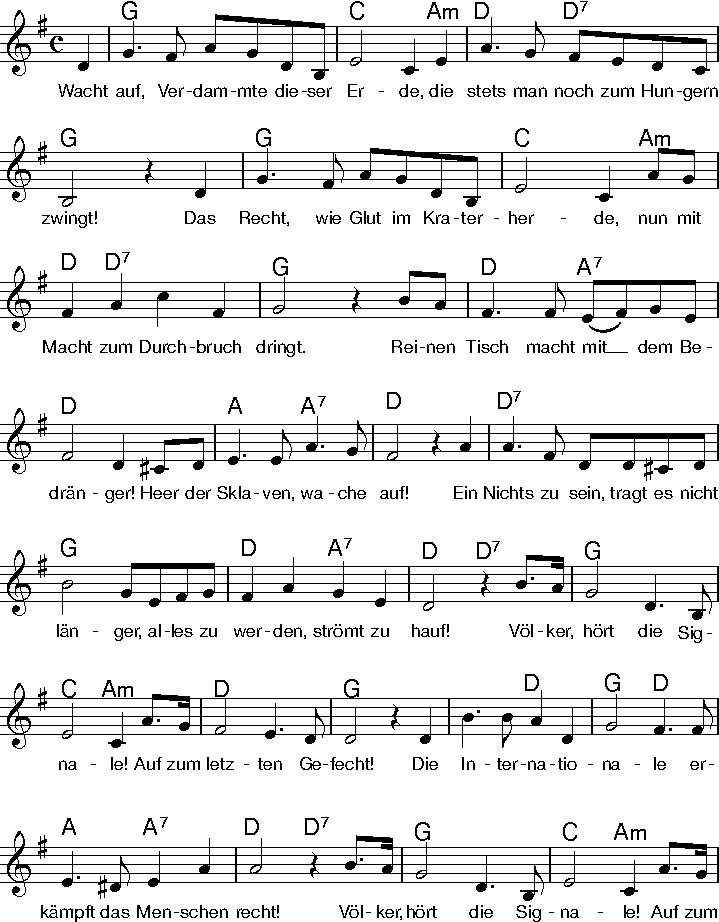
\includegraphics[width=1\textwidth]{Noten/Lied023a.pdf} 	

\beginverse*
\endverse
\centering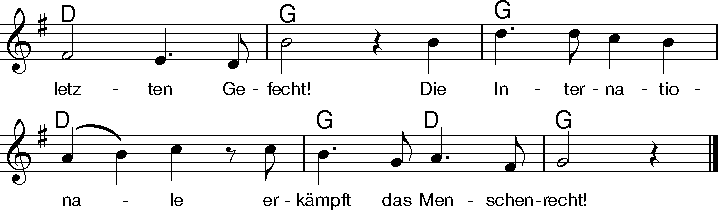
\includegraphics[width=1\textwidth]{Noten/Lied023a_1.pdf}	

\beginverse
Es \[G]rettet uns kein höh'res \[C]Wesen, kein \[D]Gott, kein \[D7]Kaiser noch Tri\[G]bun.
Uns \[G]aus dem Elend zu er\[C]lösen, können \[D]wir nur \[D7]selber \[G]tun.
\[D]Leeres Wort: Des \[A7]Armen \[D]Rechte! Leeres \[A]Wort: Des \[A7]Reichen \[D]Pflicht!
Un\[D7]mündig nennt man uns \[G]Knechte! Duldet die \[D]Schmach nun \[A7]länger \[D]nicht!\[D7]
\endverse

\beginchorus

Völker, \[G]hört die Sig\[C]nale, auf zum \[D]letzten Ge\[G]fecht!
Die Inter\[D]natio\[G]na\[D]le er\[A]kämpft das \[A7]Menschen\[D]recht\[D7]!
Völker, \[G]hört die Sig\[C]nale, auf zum \[D]letzten Ge\[G]fecht!
Die \[G]Internatio\[D]nale er\[G]kämpft das \[D]Menschen\[G]recht!
\endchorus

\beginverse
In ^Stadt und Land, ihr Arbeits^leute, sind ^wir die ^stärkste der Par^tei'n.
Die ^Müßiggänger schiebt bei^seite! Diese ^Welt muss ^unser ^sein!
Unser ^Blut ^sei nicht mehr der ^Raben und der ^mächt'gen ^Geier ^Fraß!
Erst ^wenn wir sie vertrieben ^haben, dann scheint die ^Sonn' ohn' ^Unter^lass^!
\endverse

\renewcommand{\everychorus}{\textnote{\bf Refrain (wdh.)}}
\beginchorus
\endchorus

\endsong

\beginscripture{}
Die Internationale ist das weltweit am weitesten verbreitete Kampflied der sozialistischen Arbeiterbewegung. Sie entstand im Zuge der Pariser Kommune von März bis Mai 1871, der ersten als proletarisch-sozialistisch geltenden Revolution.
\endscripture
